\begin{figure}[H]
	\begin{subfigure}{0.5\textwidth}
		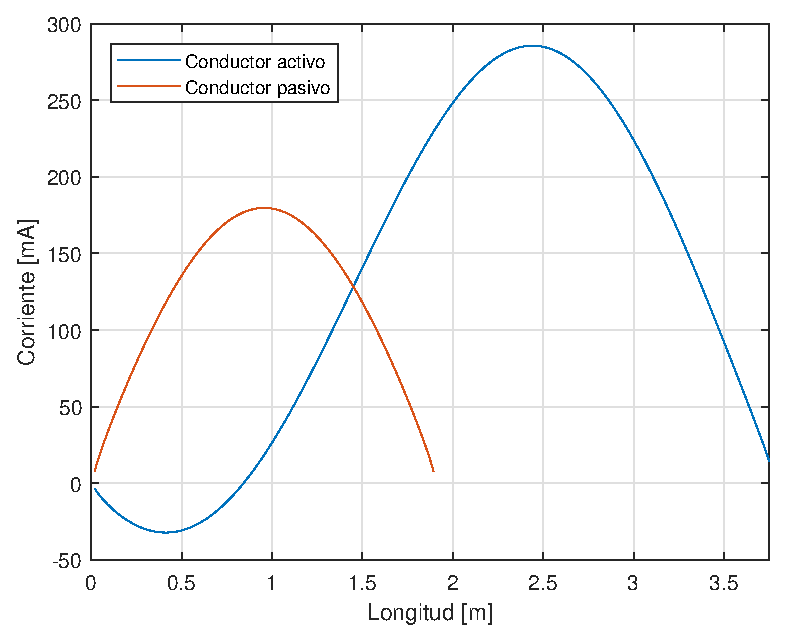
\includegraphics[scale=0.6]{imagenes/i_real_80.eps}
		\caption{Parte real.}
		\label{fig.i_real_80}
	\end{subfigure}
	\quad
	\begin{subfigure}{0.5\textwidth}
		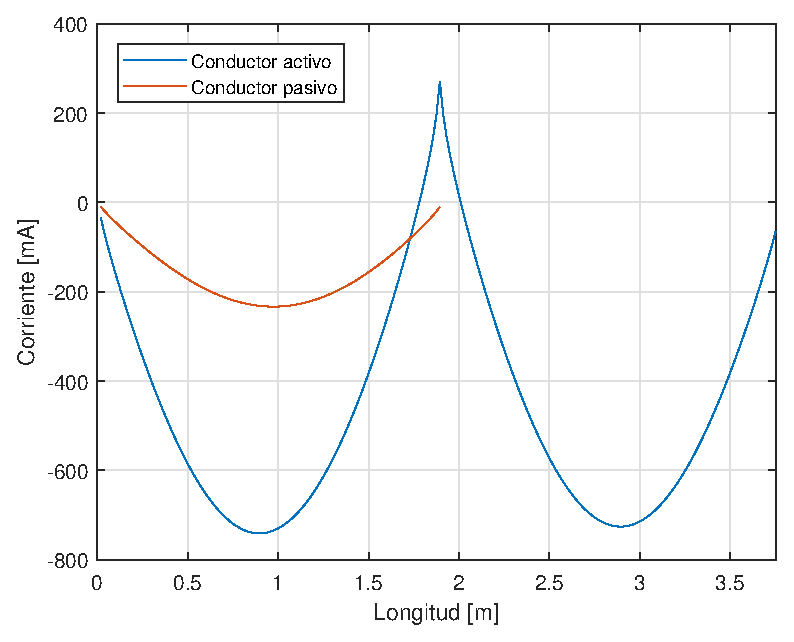
\includegraphics[scale=0.6]{imagenes/i_imag_80.eps}
		\caption{Parte imaginaria.}
		\label{fig.i_imag_80}
	\end{subfigure}
	\quad
	\begin{subfigure}{0.5\textwidth}
		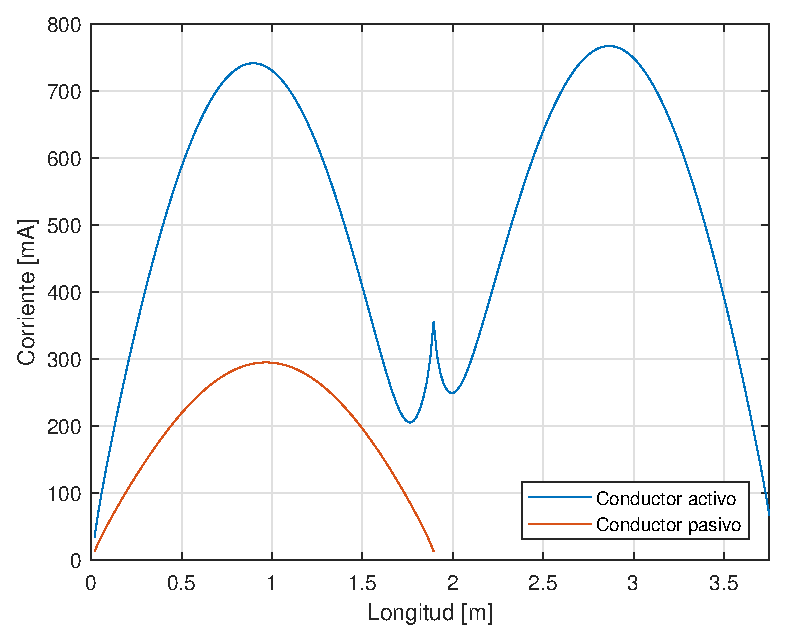
\includegraphics[scale=0.6]{imagenes/i_mag_80.eps}
		\caption{Magnitud.}
		\label{fig.i_mag_80}		
	\end{subfigure}
	\quad
	\begin{subfigure}{0.5\textwidth}
		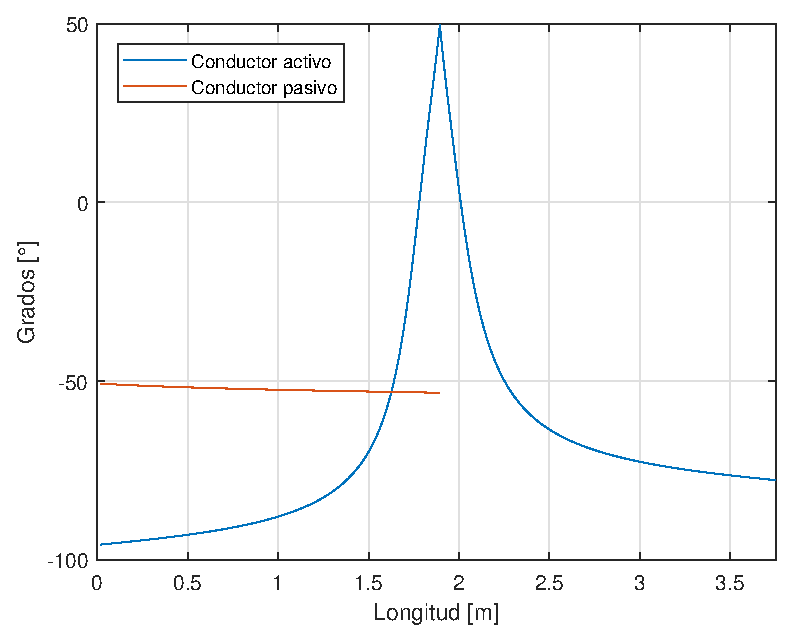
\includegraphics[scale=0.6]{imagenes/i_fase_80.eps}
		\caption{Fase.}
		\label{fig.i_fase_80}		
	\end{subfigure}
	\caption{Corriente para la frecuencia mínima $f = \SI{80}{\mega\hertz}$}
	\label{fig.i_80}	
\end{figure}

En las figuras \ref{fig.i_80} se muestra la corriente para $f=\SI{80}{\mega\hertz}$ en el conductor activo y en uno de los conductores pasivos. Se eligió el que se encuentra a la derecha del mismo a una distancia de $\lambda/2$. Como era de esperarse, la magnitud de la corriente es mayor en el conductor activo que en el pasivo. La diferencia de magnitud de las corrientes máximas entre ambos conductores es de aproximadamente $\SI{440}{\milli\ampere}$. La fase del conductor pasivo se mantiene prácticamente constante, mientras que en conductor activo cambia drásticamente en la mitad de la longitud del mismo ($\SI{1.9}{\meter}$) y luego tiende a acercarse a su valor inicial.

\begin{figure}[H]
	\begin{subfigure}{0.5\textwidth}
		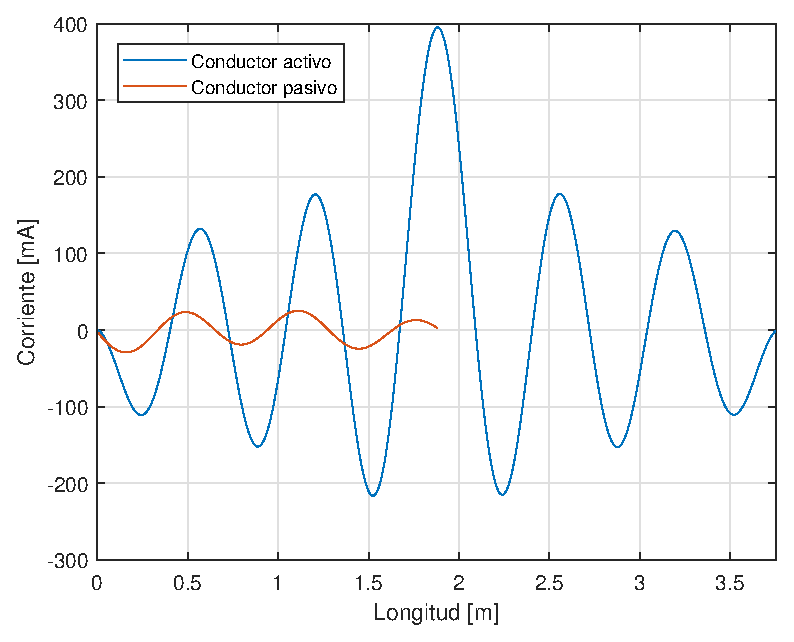
\includegraphics[scale=0.6]{imagenes/i_real_480.eps}
		\caption{Parte real.}
		\label{fig.i_real_480}	
	\end{subfigure}
	\quad
	\begin{subfigure}{0.5\textwidth}
		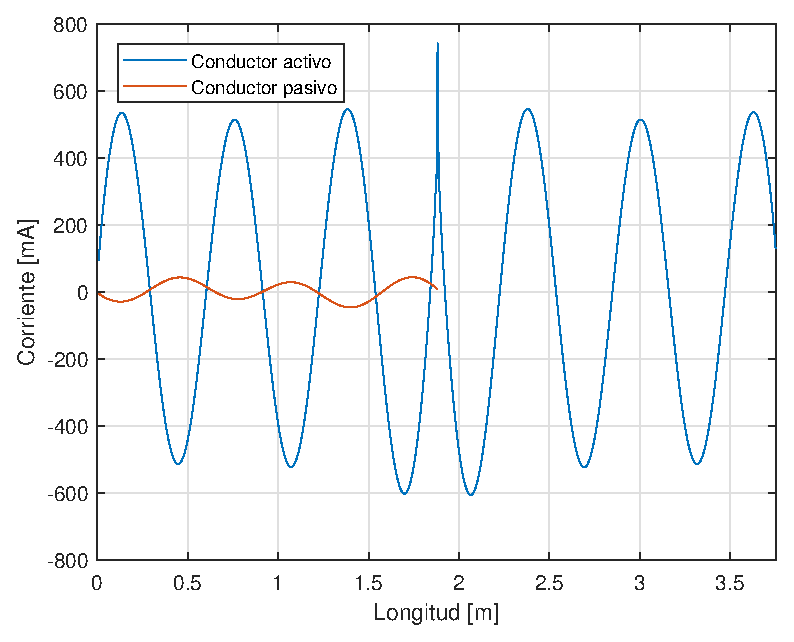
\includegraphics[scale=0.6]{imagenes/i_imag_480.eps}
		\caption{Parte imaginaria.}
		\label{fig.i_imag_480}
	\end{subfigure}
	\quad
	\begin{subfigure}{0.5\textwidth}
		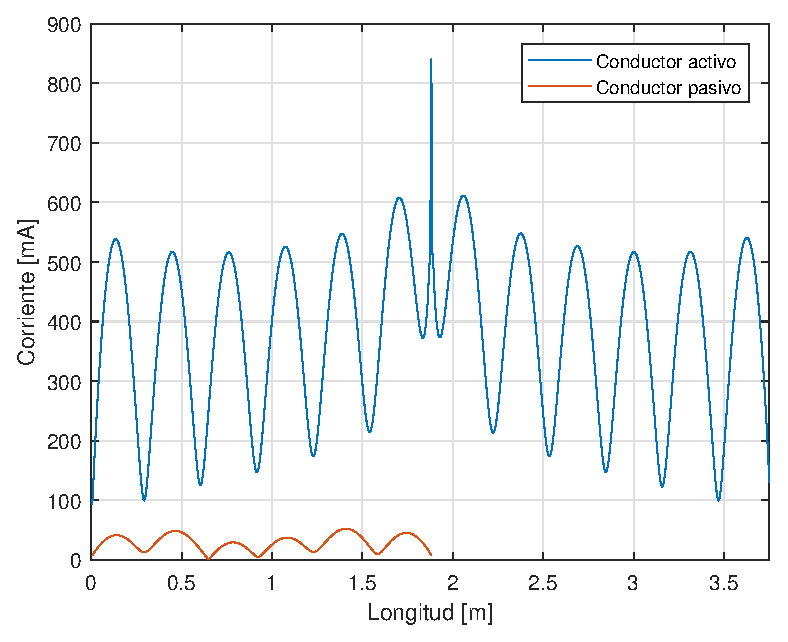
\includegraphics[scale=0.6]{imagenes/i_mag_480.eps}
		\caption{Magnitud.}
		\label{fig.i_mag_480}
	\end{subfigure}
	\quad
	\begin{subfigure}{0.5\textwidth}
		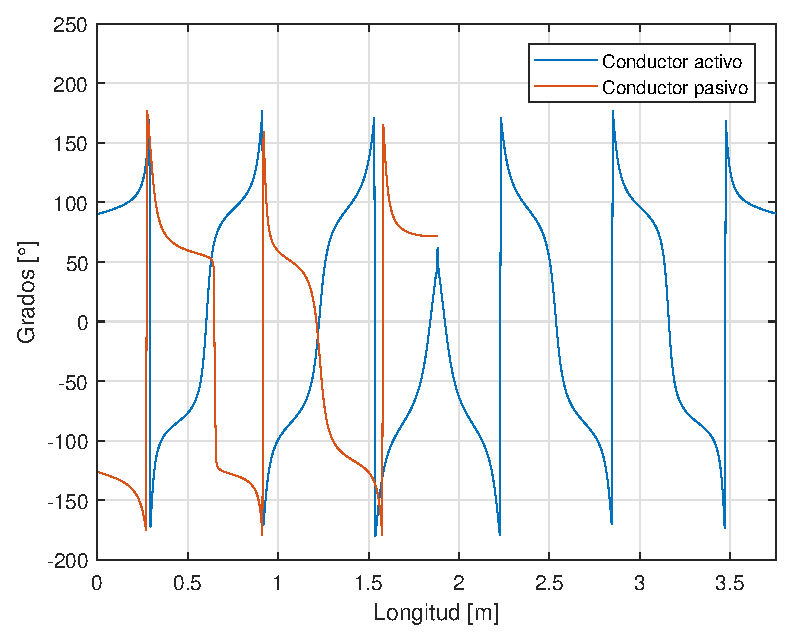
\includegraphics[scale=0.6]{imagenes/i_fase_480.eps}
		\caption{Fase.}
		\label{fig.i_fase_480}
	\end{subfigure}
	\caption{Corriente para la frecuencia máxima $f = \SI{480}{\mega\hertz}$}
	\label{fig.i_480}
\end{figure}


Análogamente se realizaron los gráficos para la máxima frecuencia. La diferencia de magnitud de las corrientes máximas entre ambos conductores es de $\SI{500}{\milli\ampere}$. Se observa que la corriente en el conductor pasivo se encuentra en contrafase al activo. Al comparar las figuras \ref{fig.i_mag_80} y \ref{fig.i_mag_480} se aprecia que entre $\SI{1.8}{\meter}$ y $\SI{2}{\meter}$, la magnitud de la corriente del conductor activo para $f=\SI{80}{\mega\hertz}$ es mínima, mientras que para $f=\SI{480}{\mega\hertz}$ es máxima.